\section{Feature Preserving Curved Shell}


\begin{figure}
    \centering
    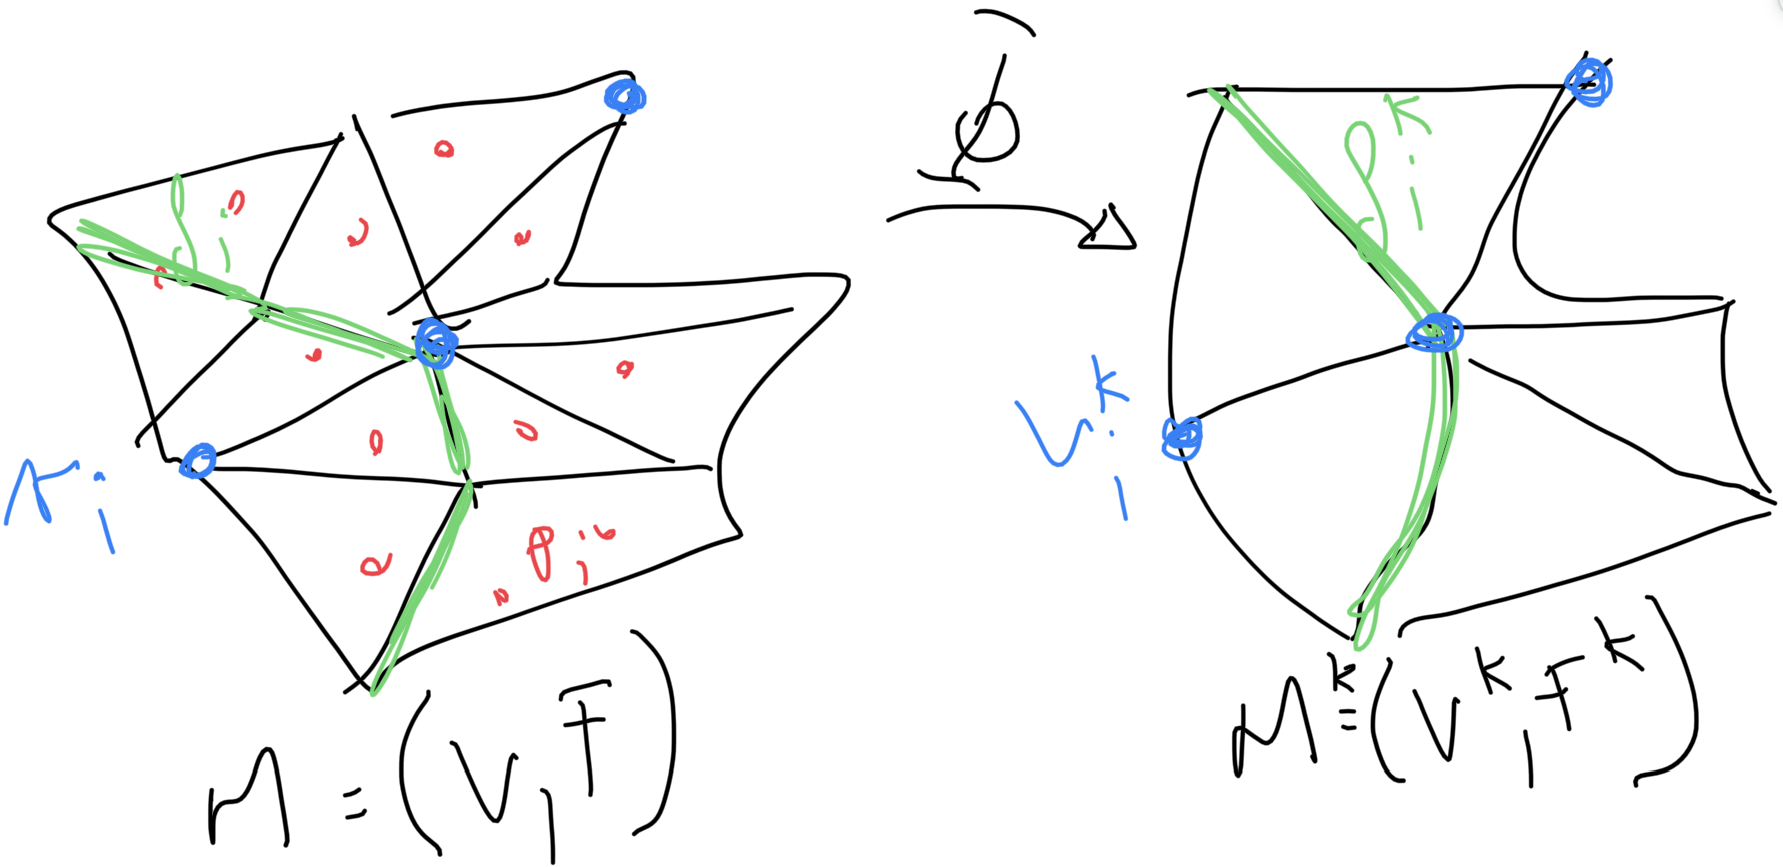
\includegraphics[width=.7\linewidth]{curve_meshing_in_shell_tex/figs/input-output}
    \caption{Input triangle mesh with features and output curved mesh with feature preserved equipped with bijective map $\phi^k$.}
    \label{bichon:fig:input-output-feature}
\end{figure}

We are now ready to extend the previous construction to features. We modify the input to additionally include a set of feature edges $f_i\in\F$ and feature vertices $v_i\in\V$ such that no triangle in $F$ has more than one feature edge (Figure~\ref{bichon:fig:input-output-feature} left). (This property can be satisfied on any generic mesh by performing 1-to-3 refinement on every triangle with more than one feature edge). Since the input has features, the output curved mesh $\M^k$ will also have curved features edges $f_i^k\in\F^k$, feature vertices $v_i^k\in\V^k$, and the bijective map $\phi^k$ preserves features by bijectively mapping $\F$ to $\F^k$ and $\V$ to $\V^k$. Our methods makes no assumption on the topology and ``quality'' of the features, if the features are reasonable it will produce an high-quality mesh while if the features are close our algorithm will preserve them and have a low quality surface (Figure~\ref{bichon:fig:bad-features}).

\begin{figure}
    \centering
    % \includegraphics{}
    \TODO{left model with good features and surface energy, middle more features, right many more features}
    \caption{Example of a model with good features (left), as we increase the number of features (middle and right) our algorithm will preserve them all and the quality of the surface will suffer.}
    \label{bichon:fig:bad-features}
\end{figure}



\begin{figure}
    \centering
    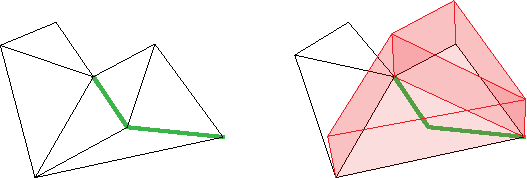
\includegraphics[width=.6\linewidth]{curve_meshing_in_shell_tex/figs/not-feat-pres}
    \caption{Input feature is not preserved after traditional shell simplification.}
    \label{bichon:fig:not-feat-pres}
\end{figure}

The previous construction generates valid curved tetrahedral meshes and the bijective map $\phi^k$ based on the construction of~\cite{jiang2020bijective}. However the shell construction cannot coarsen features or open boundaries; the authors suggest to freeze them. For instance, when performing an edge collapse on the feature the new coarse edge (orange) will not map to the feature (green) anymore (Figure~\ref{bichon:fig:not-feat-pres}). 
To ensure feature preservation we extend Definition~\ref{def:curved-mesh}.
\begin{definition}\label{def:curved-features}
We call a curved mesh $\M^K$ and its mapping $\phi^k$ from $\M$ \emph{valid and feature preserving} if they are valid (Definition~\ref{def:curved-mesh}) and $\phi^k$ bijectively maps $\F$ to $\F^k$ and $\V$ to $\V^k$
\end{definition}
As for the non-feature preserving case we always aim to maintain a valid feature preserving $\M^k$.


\begin{figure}
    \centering
    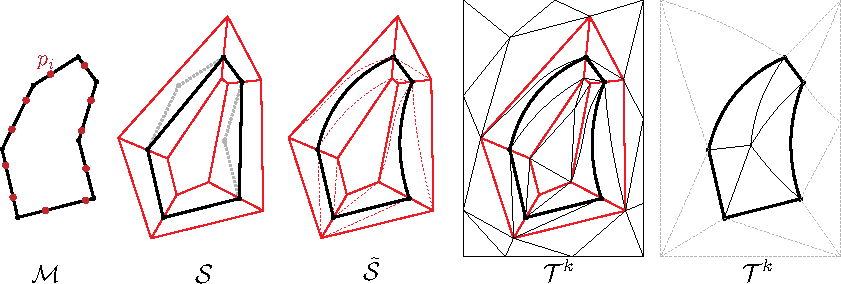
\includegraphics[width=\linewidth]{curve_meshing_in_shell_tex/figs/pipeline}
    \caption{Overview of the construction of the first stage of our pipeline}
    \label{bichon:fig:stage-1}
\end{figure}

To account for features we propose to change the prismatic map $\Pi$, that is we only need to change the first stage. This is done in two phases (Figure \ref{bichon:fig:stage-1}): input features snapping (Section~\ref{sec:snapping}) and prism grouping (Section~\ref{sec:macro}). The first phase modifies $\M$ to ``straighten'' the feature to ensure that the coarse prismatic projection preserves them and construct a mapping $b$ between the straighten mesh $\bar\M$ and $\M$. The second phase groups prisms into \emph{macro} prisms to further coarsen the shell.

The outcome of is a \emph{valid} shell $\PS$ with respect to the straighten surface $\bar\M$ (i.e., $\bar\M$ is a section $\PS$) that preserve features, the prismatic projection $\Pi$, and the bijective map $b$ that can be directly used in the curved pipeline (Section~\ref{sec:curved-pipeline}). That is the mapping  $\phi^k$ will be defined as $\phi^k = b \circ \Pi \circ \xi^k$.


\begin{figure}
    \centering
    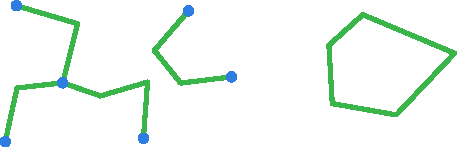
\includegraphics[width=0.5\linewidth]{curve_meshing_in_shell_tex/figs/feat-gr}
    \caption{The input edges feature (green) are grouped together in poly-lines and categorized in graph (left) and circles (right). For every graph we add the nodes (blue) to the set of feature vertices.}
    \label{bichon:fig:feat-gr}
\end{figure}

\paragraph{Feature Grouping.}
The first step of our pipeline consists of grouping successive edges $f_i\in\F$ into poly-lines and identifying two categories: loops and graphs (Figure~\ref{bichon:fig:feat-gr}). For every graph, we identify its nodes and add them as feature vertices. In other words, we add to $\V$ all the end-points and junction of poly-lines.


%%%%%%%%%%%%%%%%%%%%%%%%%%%%%%%%%%%%%%%%%%%%%%

\subsection{Feature straightening.}\label{sec:snapping}
To allow feature coarsening we propose to straighten $\M$ to ensure that all features are collinear. In other words, we build, together with the shell $\PS$, a mesh $\bar\M = (\bar V,F)$ (i.e., a mesh with the same connectivity $F$ of $\M$) and features $\bar \F$ such that every triangle of $\bar \M$ has a positive area, $\bar \M$ is a section of $\PS$, and the features in $\bar\F$ are collinear. In such a way the mapping $b$ is trivially defined as piecewise affine ($\bar\M$ and $\M$ share the same connectivity) and it locally injective as long as all the triangles on $\bar\M$ have positive area. Global bijectivity of $b$ follows from the fact that the shell prevents self-intersections of $\bar\M$ \TS{check me}.


Our goal is to construct a mesh $\bar\M$ with straight features. We start with $\bar\M = \M$ as in the beginning all prism of $\PS$ cover at most one feature edge. Let $\bar f^1 = \{\bar f_i^1\}, i=1,\dots,n$ and $\bar f^2 = \{\bar f_i^2\}, i=1,\dots,k$ two chain of features edge belonging to the same feature $\bar f \in \bar\F$.
For every local operation acting on a feature $\bar f_1$ and $\bar f_2$ (e.g., smoothing will ``move'' some edges from $\bar f_1$ to $\bar f_2$, collapse will merge all edges in a unique feature) we first construct the new feature $\bar f^n = \{\bar f_i^n\}, i=1,\dots,k$ such that the segments $(\bar f_i^n, \bar f_{i+1}^n)$ are collinear and their length is proportional to $( f_i, f_{i+1})$ (the feature vertices in the input mesh $\M$), that this we use arc-length cross parameterization from $f$ to $\bar f^n$. Moving vertices of $\bar f^n$ will also move the vertices of $\bar\M$ thus straighten the mesh as the local operations proceeds. After the construction of $\bar f^n$ we check if the newly constructed $\bar\M$ is still a section of $\PS$ and if the new triangles have area larger than $10^{-10}$ (as predicates for strictly positive do not exits\TS{true?}\ZJ{I think it exists. zero area is colinear check.}).


\begin{figure}
    \centering
    % \includegraphics[width=.5\linewidth]{curve_meshing_in_shell_tex/figs/zig}
    \TODO{add example of failed snapping}
    \caption{Examples where snapping a feature is not possible.}
    \label{bichon:fig:snapping-fail}
\end{figure}

\DP{This is is not a limitation, I think we need to change the pitch, we are trying to simplify them, it is not expected that they will all be straight. Let's discuss}\TS{I rephrased, it is not a limitation, your are right, is it better?}
Note that not all feature can be straighten (Figure~\ref{bichon:fig:snapping-fail}); for instance if a triangle has three feature vertices (the snapped feature will result on a degenerate triangle, thus $b$ will not be bijective) or if the snapping flips the normal ($\bar\M$ will not a section of $\PS$).

%%%%%%%%%%%%%%%%%%%%%%%%%%%%%%%%%%%%%%%%%%%%%%

\begin{figure}
    \centering
    \includegraphics[width=.5\linewidth]{curve_meshing_in_shell_tex/figs/zig}
    \caption{Illustration of a macro prism.}
    \label{bichon:fig:zig}
\end{figure}
\subsection{Macro Projection Operator.}\label{sec:macro}
To allow for more coarsening where snapping is not possible we propose to ``group'' prism next to a feature into one big macro-prism.
Let $P$ a prism adjacent to a feature poly-line $f\in\bar\F$ (possibly straightened) defined as a chain of $n$ oriented vertices $\bar f_i, i=1,\dots,n$. The macro-prism $P$ is defined as the union of the $n-1$ \emph{sub-prisms} $P_i$ (Figure~\ref{bichon:fig:zig}) with middle surface $(v_1, \bar f_i, \bar f_{i+1})$. The macro projection operator for $P$ is simply defined as the union of the of the sub prismatic maps over each sub-prism $P_i$. We note that this definition does not ensure that the top and bottom surface of the macro-prism are flat.\DP{why is this important?}

% \begin{theorem}\label{th:bijective}
% The projection operator $\Pi$ defined as the \TS{union?} of projection operators (possibly radial) $\Pi_P$ is bijective if (1) the volume of every prism $\Pi_P$ and sub-prism $P_i$ is positive and (2) the top and bottom surface are intersection free.
% \end{theorem}
% \begin{proof}
% It trivially follows from other paper\TODO{check which theorem}.
% \end{proof}

To ensure the \ps{} with macro-prisms is valid we need ensure that $\Pi$ is bijective and that the normal condition holds for every prism and sub-prism; which is equivalent to ensure that for every prism (including sub-prisms) the shell is valid.
% As in~\cite{jiang2020bijective}, for every prism (including sub-prsims)  we check for positivity of the volume of the by ensuring that the tetrahedral decomposition has positive volume, use collision detection to check if the top and bottom are intersection free, and ensure that normal condition holds. This stage ensure that $\Pi$ satisfies the first two invariants.

\DP{This is cryptic.}\TS{better?}
The initial shell in \cite{jiang2020bijective} is a valid feature preserving shell, as all feature poly-lines $\bar f_i$ are composed by only two vertices (i.e., the macro-prisms are made of only one prism). We extend the local operation to account macro-prism construction: a collapse of a feature, requires to take the union of the prisms; while a split (or a smoothing) only requires splitting (or sliding a vertex) a macro-prism (Appendix~\ref{app:local-ops}).


\begin{figure}
    \centering
    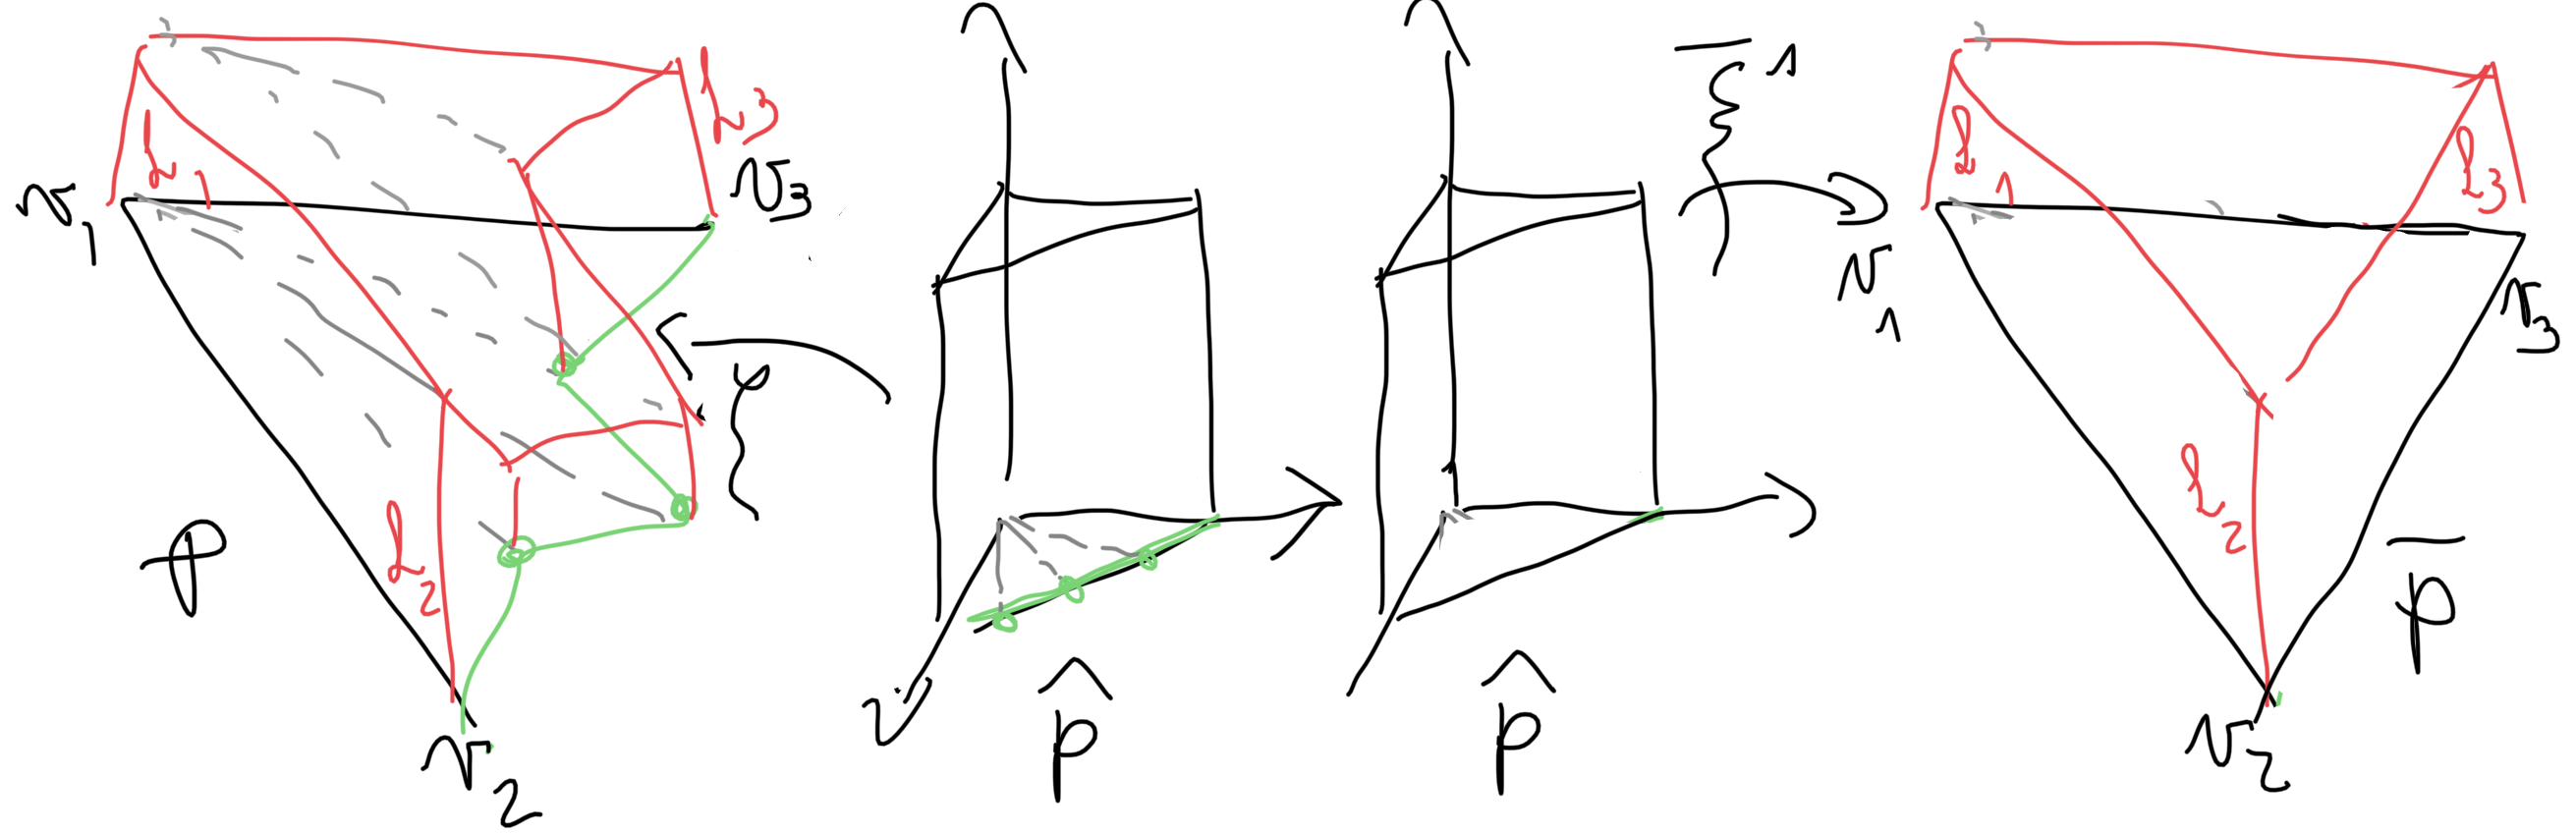
\includegraphics[width=\linewidth]{curve_meshing_in_shell_tex/figs/mappings}
    \caption{Example of mapping from $P$ to $\bar P$ passing through a reference prism $\hat P$.}
    \label{bichon:fig:ref-mapping}
\end{figure}